\chapter{Implementazione}

\paragraph{Teconologie usate}
    Il sistema \`e stato implementato in Java usando Eclipse come ambiente di sviluppo.
  
  \section{Algoritmo di riconoscimento della respirazione}
    Le fasi di cui si compone l'algoritmo di riconoscimento della respirazione ad un alto livello di astrazione sono illustrate nel diagramma seguente:
    \begin{center}
      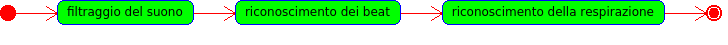
\includegraphics[width=0.9\textwidth,height=0.05\textheight]{./algoritmodiriconoscimentodellarespirazione.png}
    \end{center}

      \paragraph{Filtraggio del segnale audio}
	\begin{wrapfigure}{r}{0.3\textwidth}
	  \begin{center}
	    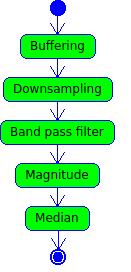
\includegraphics{./filtraggioActivity.png}
	    % onsetActivityDiagram.png: 322x477 pixel, 96dpi, 8.52x12.62 cm, bb=0 0 241 358
	  \end{center}
	  \caption{Diagramma di attivit\`a della fase di filtraggio}
	  \label{filterActivity}
	\end{wrapfigure}
	Il segnale attraversa la successione di fasi a cascata rappresentate nella figura \ref{filterActivity}. 
	Ogni filtro \`e implementato in modo simile a quanto specificato dall'interfaccia $InputStream$ di Java. 
	Siamo davanti ad un tipico caso di design di tipo \emph{pipeline} in quanto l'output di un filtro \`e l'input del filtro successivo(eccetto che per l'ultimo filtro). 
	Il segnale audio, anche nel caso in cui venga letto da un file, \`e trattato come uno \emph{stream} di dati. 
	Pi\`u in dettaglio le fasi di filtraggio sono le seguenti:
      \paragraph{$Buffering/Windowind$}
	Questa fase \`e necessaria in quanto alcuni dei filtri successivi lavorano su blocchi di input e non sul singolo campione. 
	Inoltre la presenza del buffer pu\`o diminuire il tempo totale di elaborazione.
	In questo caso l'input \`e letto da un file quindi non ci sono problemi di overflow.
	Una condizione sufficiente affinch\`e il software rispetti i propri requisiti real time \`e che la velocit\`a di elaborazione sia sempre maggiore di: un secondo di segnale fratto un secondo di tempo di elaborazione. 
      \paragraph{$Downsampling$}
	La sequenza di campionamento viene ridotta con lo scopo di aumentare l'efficienza delle fasi successive dell'algoritmo. 
	Gli spettri di potenza dei suoni respiratori e dei suoni cardiaci hanno frequenze al di sotto dei $500Hz$. 
	Quindi si pu\`o abbassare la frequenza di campionamento a $1000Hz$ in quanto una larghezza di banda di $500Hz$ \`e adeguata a catturare i suoni respiratori\cite{ASPODUOCSS}. 
      \paragraph{$Bandpass filtering$}
	Questo filtro lascia passare solo i suoni che si trovano nella banda di frequenza dai $100$ ai $1500Hz$, il risultato \`e un suono nel quale sono pi\`u facilmente distinguibili i suoni normali della respirazione. 
	Inoltre questo filtro elimina anche alcuni suoni respiratori anormali e parte dei suoni cardiocircolatori.
	Questo filtro \`e implementato grazie alle librerie JSTK reperite all'indirizzo \cite{jstk}. 
	JSTK sta per Java speech toolkit e fornisce tra le altre cose una libreria di tecniche usate per il riconoscimento vocale. 
	La libreria \`e rilasciata secondo la licenza GPLv3.
      \paragraph{$Magnitude filtering$}
	Questo filtro semplicemente prende il valore assoluto del segnale.
      \paragraph{$Median filtergin$}
	Questo \`e un classico filtro a mediana con finestra rettangolare di dimensione $10ms$ e serve per smorzare i suoni accidentali che hanno una intensit\`a relativamente alta rispetto al suono respiratorio e una durata relativamente bassa rispetto alla durata delle fasi respiratorie.

  \section{Algoritmo di beat detection}

    L'algoritmo di beat detection scelto \`e un basato su caratteristiche esplicite del segnale, prese sia dal dominio del tempo che dal dominio delle frequenze. Il thresholding \`e adattativo.
    Scegliamo la dimensione di un blocco in modo tale che contenga $4s$ di campioni dell'input. 
    Mentre scegliamo una dimensione della finestra pari a $10ms$. 
    Sia $w[1...n]$ una finestra all'interno di un blocco di campioni di suono filtrato, definiamo l'energia del suono della finestra $w$ come:
    \[
      \sum_{i=1}^{n} w[i]^{2}
    \]
    definiamo invece l'energia media locale come 
    \[
      \sum_{i=1}^{m} sb[i]^{2}
    \]
    $sb$ \`e un buffer che memorizza gli ultimi valori della media dell'energia locale. 
    Il buffer ha la dimensione adatta ad ospitare i valori relativi ad un blocco.
    % Un beat \`e una grande variazione nell'energia del suono. 
    Un modo semplice per il beat detection \`e la ricerca di picchi nell'energia del suono. 
    In questo modello ci proponiamo di riconoscere le variazioni di energia attraverso il calcolo dell'energia istantanea in una finestra di segnale delle dimensioni di $10ms$ e il confronto di questa con la media dell'energia di un blocco di al pi\`u $4s$ del segnale. 
    Non calcoliamo la media su tutto l'input disponibile perch\'e ci possono essere dei cambiamenti notevoli nel suono della respirazione su un periodo di tempo lungo. 
    Fatte queste premesse possiamo dire che riconosciamo un beat solo quando l'energia istantanea \`e superiore all'energia media. 

    \incmargin{1em}
    \restylealgo{boxed}\linesnumbered
    \begin{algorithm}
      \dontprintsemicolon
      \SetVline
      \SetKwFunction{getAverageLocalEnergy}{getAverageLocalEnergy}
      \SetKwFunction{getInstantSoundEnergy}{getInstantSoundEnergy}
      \SetKwFunction{Write}{write}
      \SetKwFunction{Init}{init}
      \SetKwFunction{Clear}{clear}
      \SetKwFunction{Add}{add}
      \SetKwInOut{Input}{input}
      \SetKwInOut{Output}{output}
      \caption{beat detection}
      \Input{A block of filtered sound samples}
      \Output{A sequence of boolean}
      \BlankLine
      soundEnergyHistoryBuffer.\Clear{}\;
      \ForEach{window $w$ in the input block}{
	instantSoundEnergy $\leftarrow$ w.\getInstantSoundEnergy{}\;
	averageLocalEnergy $\leftarrow$ soundEnergyHistoryBuffer.\getAverageLocalEnergy{}\;
	soundEnergyHistoryBuffer.\Write{instantSoundEnergy}\;
	\eIf{instantSoundEnergy $>$ averageLocalEnergy}{
	  beatSequence.\Add{true}\;
	}{
	  beatSequence.\Add{false}\;
	}
      \Return beatSequence\;
      }
      \label{algBeatDet}
    \end{algorithm}
    \decmargin{1em}



  \section{Riconoscimento delle apnee a rischio}
    La fase di riconoscimento del respiro prende in input le sequenze di booleani date in output dalla fase precedente. 
    Ricordiamo che un elemento della sequenza ha valore di verit\`a vero se corrisponde ad un beat altrimenti vale falso. 
    Questa fase si divide nelle due fasi seguenti.

\paragraph{Clustering}

La prima fase del riconoscimento \`e un \emph{clustering} dei dati della fase precedente. 
In questo contesto un cluster \`e una sequenza di booleani di lunghezza non nota a priori.
Un cluster non deve avere una lunghezza superiore ad una certa soglia ad esempio la lunghezza che corrisponde ad un segnale di $1s$.
% Ci sono solo due tipi di cluster: presenza di suoni respiratori (fase inspiratoria o fase espiratoria) e assenza di suoni respiratori (eventuale apnea). Definiamo il classificatore $C$ nel modo seguente:
% \begin{center}
%   \begin{tabular}{ll}
% 	$C:\tilde{x} \mapsto$ suono
%       &
% 	se $\tilde{x}$ contiene per almeno  $90\%$ beats
%     \\
% 	$C:\tilde{x} \mapsto$ silenzio
%       &
% 	altrimenti
%     \\
%   \end{tabular}
% \end{center}

Usiamo il seguente algoritmo di clustering sequenziale e con cluster sequenziali di lunghezza non nota a priori:
\incmargin{1em}
\restylealgo{boxed}\linesnumbered
\begin{algorithm}
  \dontprintsemicolon
  \SetVline
  % \SetNoline
%   \SetKwData{b}{b}
%   \SetKwData{This}{this}
%   \SetKwData{Up}{up}
  \SetKwFunction{getAverageLocalEnergy}{getAverageLocalEnergy}
  \SetKwFunction{getInstantSoundEnergy}{getInstantSoundEnergy}
  \SetKwFunction{Write}{write}
  \SetKwFunction{Init}{init}
  \SetKwFunction{Clear}{clear}
  \SetKwFunction{Add}{add}
  \SetKwFunction{DDDD}{distance}
  \SetKwInOut{Input}{input}
  \SetKwInOut{Output}{output}
  \caption{Beat clustering}
    \Input{A sequence of boolean $x_{1}, \cdots, x_{n}$}
    \Output{A clustering of the data $C_{1}, \cdots, C_{m}$}
    \BlankLine
    $m\leftarrow 1$\;
    $C_{m}.data \leftarrow \{x_{1}\}$\;
    $C_{m}.type \leftarrow x_{1}$
    \For{$i\leftarrow 2$ \KwTo $n$}{
       \eIf{($\DDDD(x_{i}, C_{m}) > $ threshold) $\vee$ ($C_{m}>maxSize$) $\vee$ $i==n$}{
 	increments $m$\;
	$C_{m}.data \leftarrow \{x_{i}\}$\;
	$C_{m}.type \leftarrow x_{i}$
       }{
 	$C_{m}.data \leftarrow C_{m}.data \cup \{x_{i}\}$\;
       }
  }
\label{clusteringSequenzialeImplementazione}
\end{algorithm}
\decmargin{1em}


La distanza tra un elemento $x_{i}$ e un cluster $C_{m}$ \`e 
% \[
%   distance(x_{i}, C_{m})= 
%   \left|x_{i} -  \displaystyle\frac{\displaystyle\sum_{j\in C_{m}} j}{|C_{m}|}\right|
% \]
\[
distance(x_{i}, C_{m})= 
 \left\{ 
    \begin{array}{ll}
 	\displaystyle\frac{beat\; count}{cluster\; size(C_{m})}
       &
 	se\; x_{i}=false
     \\\\
 	1-\displaystyle\frac{beat\; count}{cluster\; size(C_{m})}
       &
 	se\; x_{i}=true
     \\
     \end{array}
   \right.
\]

La soglia \`e di $0.7$ ed \`e stata scelta in modo empirico.



% 2. FARE UN ESEMPIO DI CLUSTERIZZAZIONE
% dmettere una immagine che mappa una sequenza di beat in una sequenza di cluster!



La fase di cluster serve per correggere eventuali falsi beat della fase precedente, ad esempio un beat che non era causato dal respiro e che non \`e stato eliminato dalla fase di filtraggio oppure serve per aggiungere beat mancanti ad esempio nel caso di una piccola apnea localizzata immediatamente dopo la fase inspiratoria e prima della fase espiratoria.


\paragraph{Riconoscimento delle apnee a rischio}

L'algoritmo considera come pausa respiratoria una sequenza non vuota di cluster $C_{1}, \cdots, C_{n}$ tale che $C_{i}.type=false$ per ogni $i$.
Appena la durata totale della pausa respiratoria supera una soglia critica, il sistema suona una allarme e si mette in attesa che l'allarme venga spenta attraverso un comando apposito dell'interfaccia utente.





\section{Complessit\`a computazionale dell'algoritmo}

Calcolare in modo preciso la complessit\`a asintotica dell'algoritmo \`e difficile perch\`e \`e difficile determinare la complessit\`a del filtro passa banda della libreria JSTK, tuttavia escludendo questa libreria, il resto dell'algoritmo \`e lineare nel numero dei campioni. 
La complessit\`a \`e relativa alla macchina virtuale Java. 










